\documentclass[11pt]{article}
\usepackage{amsmath,amssymb,amsthm}
\usepackage{graphicx}
\usepackage[margin=1in]{geometry}
\usepackage{fancyhdr}
\usepackage{float}
\setlength{\parindent}{0pt}
\setlength{\parskip}{5pt plus 1pt}
\setlength{\headheight}{13.6pt}
\newcommand\question[2]{\vspace{.25in}\hrule\textbf{#1: #2}\vspace{.5em}\hrule\vspace{.10in}}
\renewcommand\part[1]{\vspace{.10in}\textbf{(#1)}}
\newcommand\algorithm{\vspace{.10in}\textbf{Algorithm: }}
\newcommand\result{\vspace{.10in}\textbf{Result: }}
\pagestyle{fancyplain}
\lhead{\textbf{\NAME\ (\ANDREWID)}}
\chead{\textbf{Assignment\HWNUM}}
\rhead{STAT3006: Statistical Computing}
\begin{document}\raggedright
%Section A==============Change the values below to match your information==================
\newcommand\NAME{ZHANG Xinfang}  % your name
\newcommand\ANDREWID{1155141566}     % your student id
\newcommand\HWNUM{2}              % the homework number
%Section B==============Put your answers to the questions below here=======================

\question{1}{Inverse method for Poissson Distribution (25\%)} 
For discrete Poisson Distribution ($\lambda = 5$),

the p.m.f is $P(x|\lambda) = e^{-\lambda} \frac{\lambda^x}{x!}$ and
the c.d.f is $F(x|\lambda) = \sum_{t \leq x} e^{-\lambda} \frac{\lambda^t}{t!}$.

\algorithm
Inverse method for the Poisson Distribution:

To generate $X \sim F(x)$:

STEP 1: Generate $U \sim unif[0, 1]$;

STEP 2: Transform $X = F^-(U)$: if $F(x|\lambda) < U \leq F(x+1|\lambda)$, let $X = x+1$.

$\mathbf{Plot:}$

\begin{figure}[H]
    \centering
    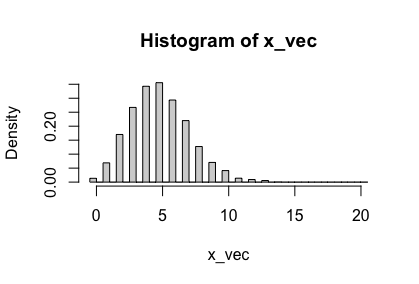
\includegraphics[width=13cm]{figures/q1_plot_new.png}
    \caption{Histogram of 5000 samples}
  \end{figure}
\question{2}{Accept-Reject method for truncated Gamma Distribution (25\%)}
For $X \sim Gamma(\frac{1}{2}, 1)I(x \geq 5)$, $f(x) = \frac{x^{-\frac{1}{2}}e^{-x}I(x\geq 5)}{\int_5^{+ \infty} y^{-\frac{1}{2}}e^{-y} dy}$.

We can define a shifted exponential distribution $g(x) = e^{-(x-5)}I(x \geq 5)$ and want to find a constant $M$ such that $f(x) < Mg(x)$ for any $x$.\\
Then $M = $ sup$ \frac{f(x)}{g(x)} = $ sup$ \frac{\frac{x^{-\frac{1}{2}}e^{-x}I(x\geq 5)}{\int_5^{+ \infty} y^{-\frac{1}{2}}e^{-y} dy}}{e^{-(x-5)}I(x \geq 5)} = \frac{5^{-\frac{1}{2}}e^{-5}}{\int_5^{+ \infty} y^{-\frac{1}{2}}e^{-y} dy}$.

\algorithm
Accept-Reject method for truncated Gamma Distribution:

To generate $X \sim F(x) = $ c.d.f of $f(x)$:

STEP 1: Generate $Y \sim g(y)$;

STEP 2: Generate $U \sim unif[0, 1]$;

STEP 3: Accept $X = Y$ if $U \leq \frac{f(Y)}{Mg(Y)}$.

$\mathbf{Proof:}$

From the choice of constant $M$, we can know that $Mg(x) \geq f(x)$. The goal of this method is 
to generate $X \sim F(x) = $ c.d.f of $f(x)$.

For the generating algorithm:

\begin{flalign*}
  P(X \leq x) &= P(Y \leq x | Y \text{ is accepted})\\
              &= P(Y \leq x | U \leq \frac{f(Y)}{Mg(Y)})\\
              &= \frac{P(Y \leq x, U \leq \frac{f(Y)}{Mg(Y)})}{P(U \leq \frac{f(Y)}{Mg(Y)})}\\
              &= \frac{\int_{- \infty}^x g(y) \int_0^{\frac{f(y)}{Mg(y)}} 1 du dy}{\int_{- \infty}^{+ \infty} g(y) \int_0^{\frac{f(y)}{Mg(y)}} 1 du dy}\\
              &= \frac{\int_{- \infty}^x g(y) \frac{f(y)}{Mg(y)} dy}{\int_{- \infty}^{+ \infty} g(y) \frac{f(y)}{Mg(y)} dy}\\
              &= \frac{\int_{- \infty}^x f(y) dy}{\int_{- \infty}^{+ \infty} f(y) dy}\\
              &= \frac{\int_{- \infty}^x f(y) dy}{1}\\
              &= F(x)
\end{flalign*}
Therefore, this AR method works.

$\mathbf{Comparison:}$

Theoretical acceptance probability:

\begin{flalign*}
  P(U \leq \frac{f(Y)}{Mg(Y)}) &= \int_{- \infty}^{+ \infty} g(y) \int_0^{\frac{f(y)}{Mg(y)}} 1 du dy\\
                               &= \frac{1}{M} \int_{- \infty}^{+ \infty} f(y) dy\\
                               &= \frac{1}{M}
\end{flalign*}
After computation, this acceptance probability is 0.184157.

The actual acceptance rate is $0.1854$, which is a little bit higher than the theoretical value.

\question{3}{Importance Sampling for Estimation (25\%)}

\part{1} 
Using 5000 samples from Q2 ($l$ = length of samples obtained in Q2), the Monte Carlo estimate is
\begin{flalign*}
  \int_5^{+ \infty} cos(x)x^{-\frac{1}{2}}e^{-x} dx &= \int_{- \infty}^{+ \infty} cos(x)\frac{x^{-\frac{1}{2}}e^{-x}I(x\geq 5)}{\int_5^{+ \infty} y^{-\frac{1}{2}}e^{-y} dy}dx \times \int_5^{+ \infty} y^{-\frac{1}{2}}e^{-y} dy\\
                                                    &= \frac{\int_5^{+ \infty} y^{-\frac{1}{2}}e^{-y} dy}{l}\sum_{i=1}^{l} cos(x_i)\\
                                                    &= 0.001708
\end{flalign*}
\part{2}
Using the same notations in Q2, we define $h(x) = cos(x)$.
\begin{flalign*}
  \int_5^{+ \infty} cos(x)x^{-\frac{1}{2}}e^{-x} dx &= \int_{- \infty}^{+ \infty} cos(x)\frac{x^{-\frac{1}{2}}e^{-x}I(x\geq 5)}{\int_5^{+ \infty} y^{-\frac{1}{2}}e^{-y} dy}dx \times \int_5^{+ \infty} y^{-\frac{1}{2}}e^{-y} dy\\
                                                    &= \int_5^{+ \infty} y^{-\frac{1}{2}}e^{-y} dy \int_{- \infty}^{+ \infty} \frac{h(x)f(x)}{g(x)} dx
\end{flalign*}
Note that $\frac{f(x)}{g(x)} \leq M < \infty$, and $E_gh^2(x) = \int_{- \infty}^{+ \infty} g(x)h^2(x) dx \leq \int_{- \infty}^{+ \infty} g(x) dx = 1 < \infty$, we can use the importance sampling as follows:

\algorithm

STEP 1: Generate $n = 5000$ samples from $g(x)$;

STEP 2: Compute the Monte Carlo estimate: 
\hspace*{3cm} $\int_{- \infty}^{+ \infty} \frac{h(x)f(x)}{g(x)} dx = \frac{\sum_{i=1}^{n} \frac{h(x_i)f(x_i)}{g(x_i)} }{n} = \frac{e^{-5}}{n \int_5^{+ \infty} y^{-\frac{1}{2}}e^{-y} dy} \sum_{i=1}^{n} cos(x_i) x_i^{-\frac{1}{2}}$

Therefore,
\begin{flalign*}
  \int_5^{+ \infty} cos(x)x^{-\frac{1}{2}}e^{-x} dx &= \int_5^{+ \infty} y^{-\frac{1}{2}}e^{-y} dy \int_{- \infty}^{+ \infty} \frac{h(x)f(x)}{g(x)} dx\\
                                                    &= \int_5^{+ \infty} y^{-\frac{1}{2}}e^{-y} dy  \frac{e^{-5}}{n \int_5^{+ \infty} y^{-\frac{1}{2}}e^{-y} dy} \sum_{i=1}^{n} cos(x_i) x_i^{-\frac{1}{2}}\\
                                                    &= \frac{e^{-5}}{n} \sum_{i=1}^{n} cos(x_i) x_i^{-\frac{1}{2}}\\
                                                    &= 0.00174
\end{flalign*}
\question{4}{Stratified Sampling (25\%)}

\part{1} 

\part{2}

\part{3} 

\end{document}
